%%%%%%%%%%%%%%%%%%%%%%%
% Comp 160, Algorithms
% Homework 0 template file
% Author: Matias Korman 
%%%%%%%%%%%%%%%%%%%%%%%

% This portion of the LaTeX document are configuration 
% You can see it as all the equivalent of "#include" in C++
\documentclass[12pt]{article}
\usepackage{graphicx}
\usepackage{tikz}
\usepackage{coffee4}
\graphicspath{ {./images/} }
% These three lines add some packages to the LaTeX.
% This is the equivalent of #include from C++ (importing known libraries)
% The libraries help inserting figures, use math statements, and so on
\usepackage{epsfig}
\usepackage{amsmath,amsthm}
\usepackage{listings}

% These lines describe the environments we will use: Lemma and Theorem
% Although may sound repetitive to declare that our lemma will be displayed as Lemma
% it is needed so that LaTeX can write documents in other languages 
\newtheorem{lemma}{Lemma}
\newtheorem{problem}{Problem}
\newtheorem{theorem}{Theorem}

% The commands below change the bold text where it says "Section" into "Question"
\usepackage{titlesec}
\titleformat{\section}
{\normalfont\Large\bfseries}{Question~\thesection:}{1em}{}

%Commands below change page margins (this much space at the titlepage, etc)
\newlength{\toppush}
\setlength{\toppush}{2\headheight}
\addtolength{\toppush}{\headsep}

%Name and subject of the class
\def\subjnum{Comp 160}
\def\subjname{Algorithms}

%Name of the student, university name and which semester
\def\doheading#1#2#3{\vfill\eject\vspace*{-\toppush}%
  \vbox{\hbox to\textwidth{{\bf} \subjnum: \subjname \hfil Erli Cai}%
    \hbox to\textwidth{{\bf} Tufts University, Fall 2020 \hfil#3\strut}%
    \hrule}}

%Command for the title of the document (Homework 0)
\newcommand{\htitle}[1]{\vspace*{1.25ex plus 1ex minus 0ex}%
\begin{center}
{\large\bf #1}
\end{center}} 


%%%%%%%%%%%%%%%%%%%%%%%%%%%%%%%%%%%%%%%%%%%%%%%%%%%%%%%%%%%%%%%%%%%
% BEGIN DOCUMENT
%%%%%%%%%%%%%%%%%%%%%%%%%%%%%%%%%%%%%%%%%%%%%%%%%%%%%%%%%%%%%%%%%%%
\begin{document}
\doheading{2}{title}{Homework 00}


%%% write your answer here


%section 1 self introductiuion
\section{Self Introduction}

%subsection 1.1 photo
\subsection{Photo}
\begin{center}
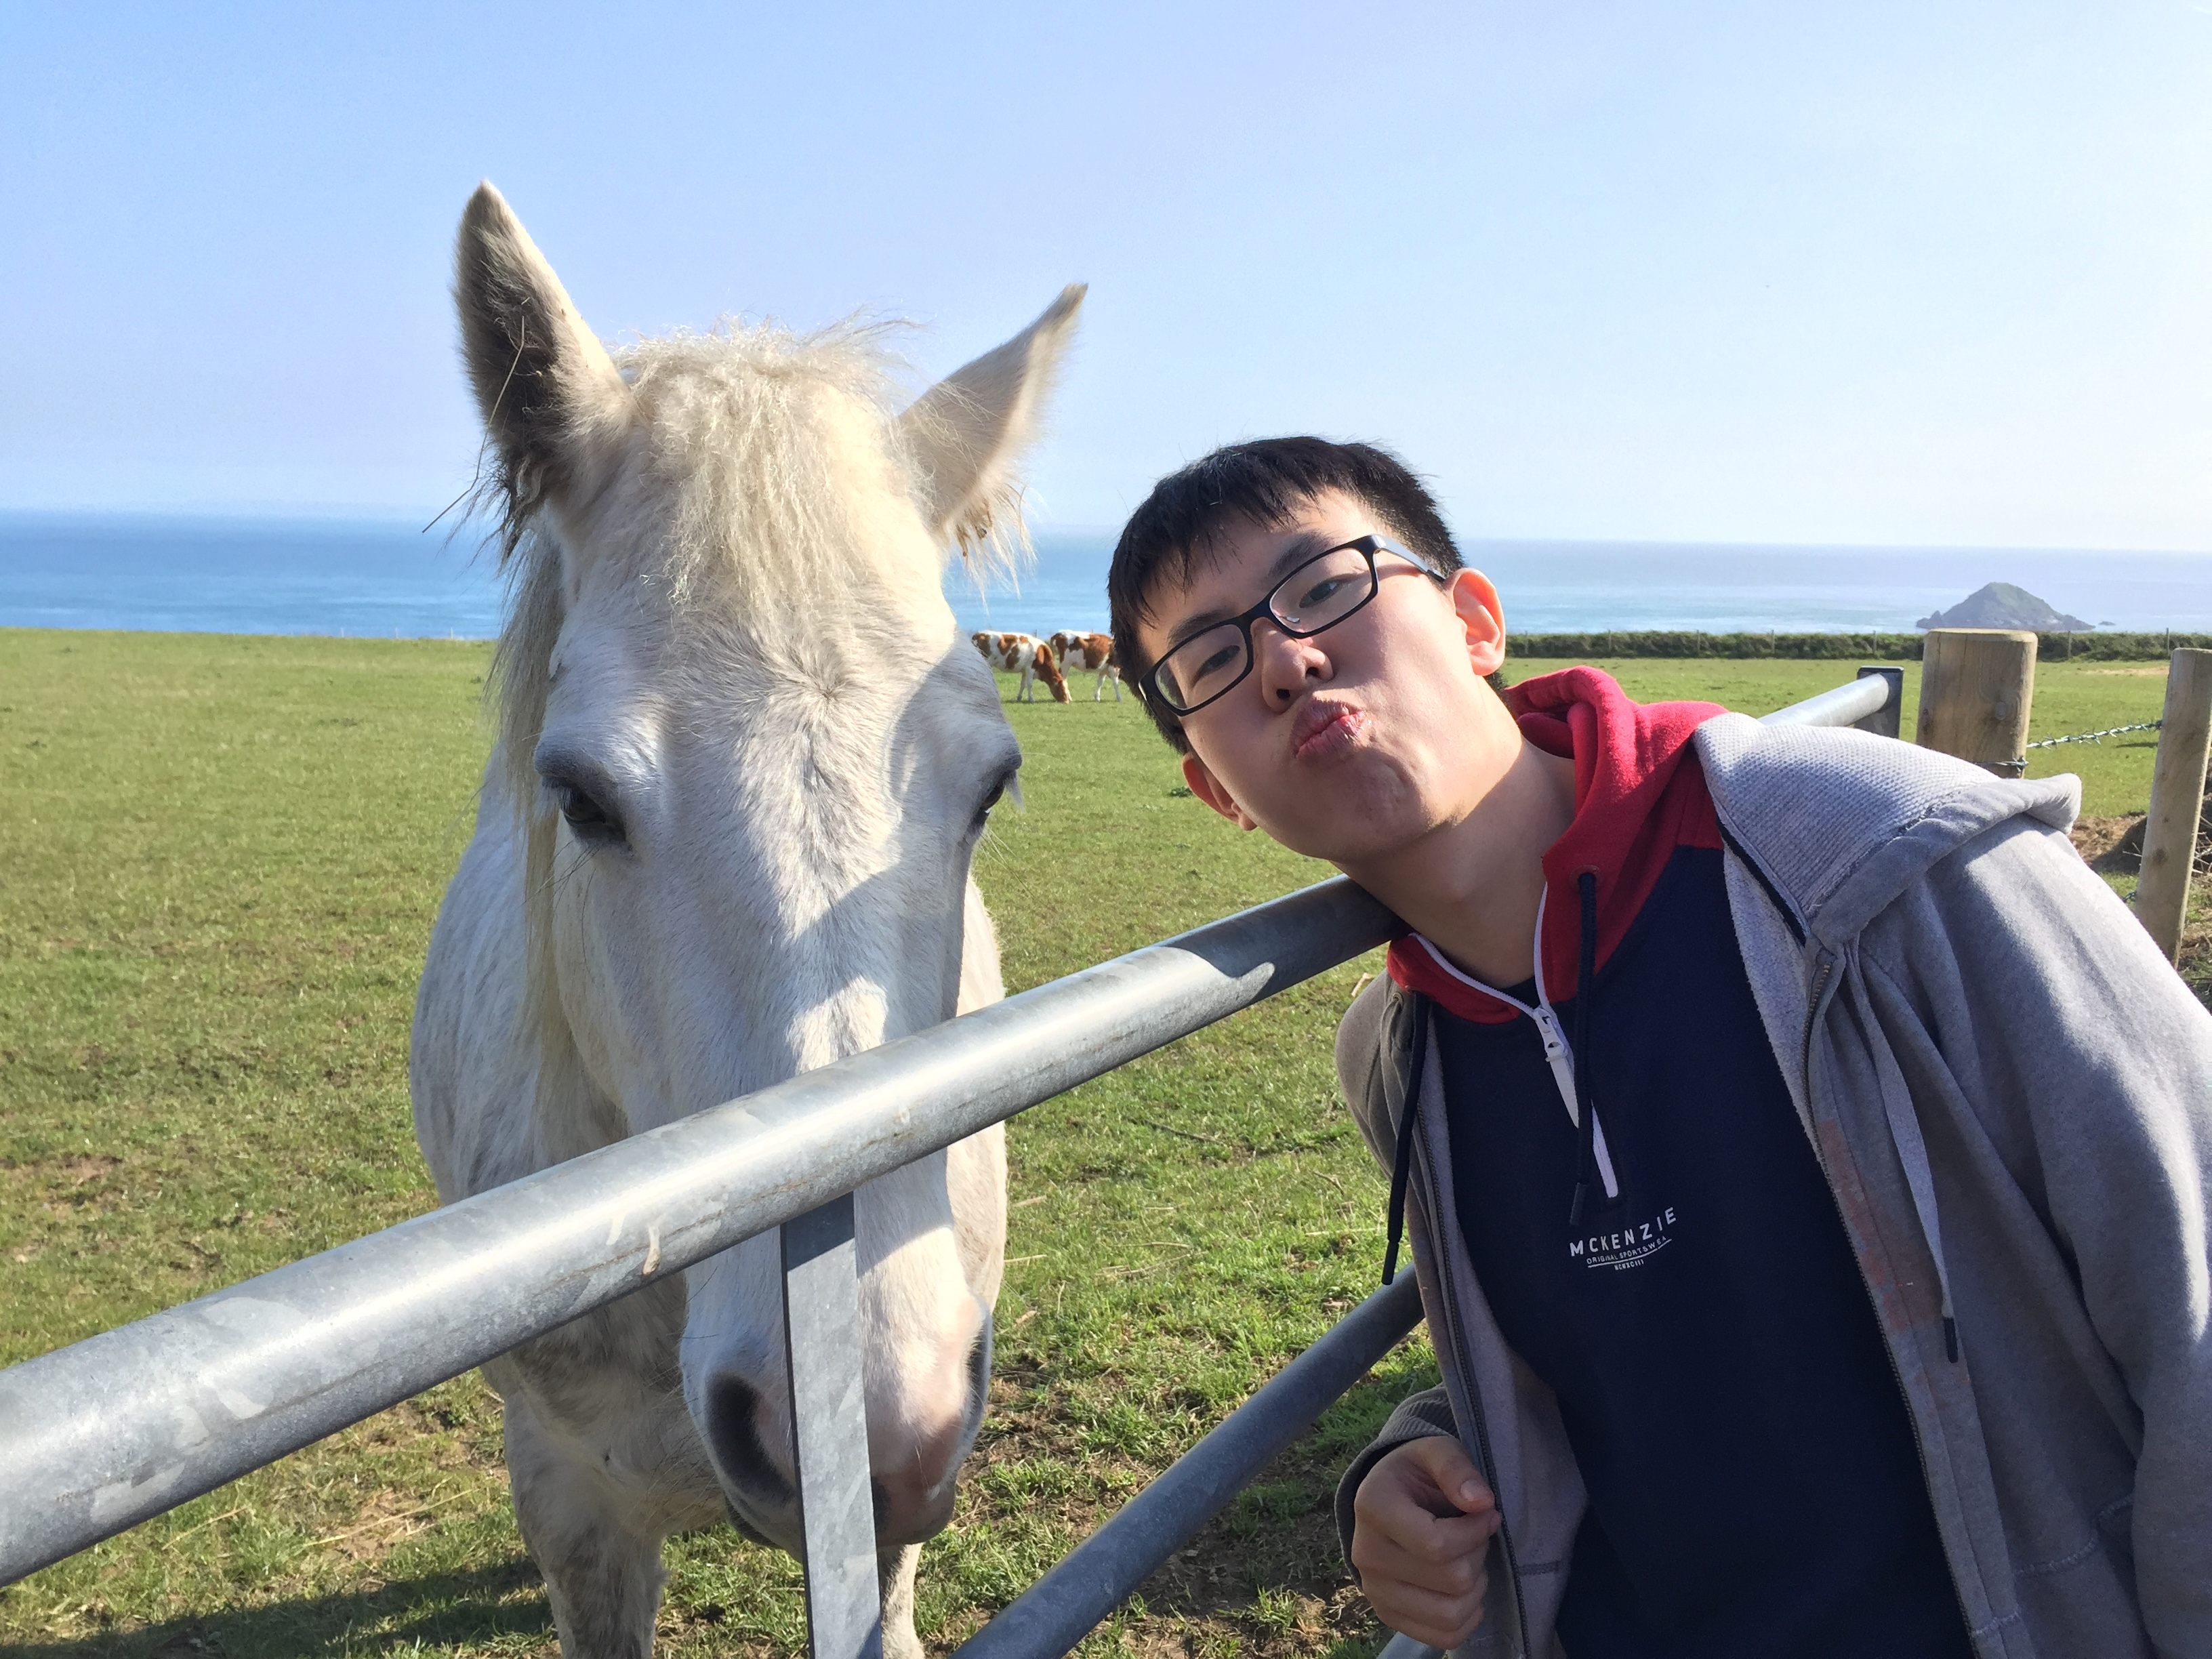
\includegraphics[width=\textwidth]{sark}
Last year at Sark Island
\end{center}

%subsection 1.2 hobbies
\subsection{Hobbies}
\begin{enumerate}
 \item Computer Games: Nobody could resist a good game with friends on weekend.
 \item Guitar: Start this hobby recently. Though not really good at it, I find myself enjoying it quite a lot.
\end{enumerate}

\pagebreak
%Section 2 Previous Knowledge
\section{Previous Knowledge}

%Known Topics
\subsection{Known Topics}
\begin{description}
 \item Big O, $\Omega, \Theta$ notation: Notations used to describe upper and lower bound of functions. 
 \item Amortisation: A way to measure the performance of an algorithm.  
\end{description}


\subsection{Familiar Topics}
\begin{itemize}
 \item  Hasing
 \item  Insertion Sort
 \item Dijkstra
 \item Kruskal's algorithm
\end{itemize}

\subsection{Unknown Topics}
\begin{itemize}
 \item  Quick sort: Always want to learn the quick sort.
 \item  Dynamic Programming: Heard of it quite a lot, but don't know that it is.
\end{itemize}
\pagebreak

\section{Proof Practice}
\begin{problem}
Design an algorithm that, given an array A of n real numbers, computes the largest value that can be obtained by multiplying all but one entry of A. You cannot use an entry more than once. Also, your algorithm is not allowed to use the division operator (explicitly or implicitly).
\end{problem}


\begin{lemma}
Let neg be the number of negative values in A. The optimal solution would ignore:\\
\begin{itemize}
 \item The largest negative if neg is odd.
 \item The smallest non-negative if not all numbers in A are negative and neg is even. (This covers the case when all numbers in A are positive)
 \item the smallest negative number if all numbers in A are negative and neg is even.
\end{itemize}
\end{lemma}
\begin{proof} 
Firstly, since positive number is always greater than negative number, we would want to result positive if it's possible. \\
Secondly, we compare the absolute value of result to decide which result is optimal. That is saying, positive result with largest absolute value is largest among positive result and negative result with smallest absolute value is largest among negative result
\begin{description}
\item When neg is odd, we have at least one negative number. In order to make the result positive, we need to ignore a negative number. To make the result optimal, we need to ignore the number with the least absolute value. In conclusion, we ignore the largest negative number.
\item When not all numbers in A are negative and neg is even, the result of multiplying all numbers in A is positive, so we want to ignore a positive number. And to make result optimal, we ignore the number with smallest absolute value, which is the smallest non-negative number.
\item  When all numbers in A are negative and neg is even, we get a negative result no matter which number we ignore. So to make the result as large as possible, we want the absolute value of result as small as possible. So we ignore the smallest negative number.
\end{description}
\end{proof}

Algorithm: Go through the list and find the number of negative number, largest negative number, smallest non negative number and smallest negative number respectively. Choose the one to ignore according to the lemma and calculate the result.\\

Justification: The lemma ensures that we choose to ignore the number that optimise the result.\\

Runtime: Go through the list would take O(n) time. Choose the number to ignore would take O(1) time. And multiply every number in the list except one would take O(n) time , so the algorithm take O(n) time.


\pagebreak

\section{Fun Challenge}
\subsection{Formula}
\begin{center}
$\sqrt{\frac{A}{B}}i = \sqrt{\frac{A}{B}e^{i\pi}}$
\end{center}

\subsection{Tables}
\begin{tabular}{|c | c | c | c | c | c|}
\hline
& Monday & Tuesday & Wednesday & Thursday & Friday\\
\hline
10:00&getup&getup&getup & getup & getup\\
\hline
24:00&go to sleep&go to sleep&go to sleep&go to sleep&go to sleep\\
\hline
\end{tabular}

\subsection{Figure}
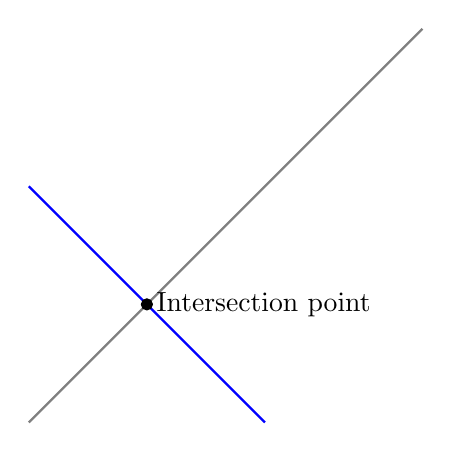
\begin{tikzpicture}
\draw[gray, thick] (0,0) -- (5,5);
\draw[blue, thick] (3,0) -- (0,3);
\filldraw[black] (1.5,1.5) circle (2pt) node[anchor=west] {Intersection point};

\end{tikzpicture}

\subsection{Command} 
\cofeAm{1}{1}{90}{5.5cm}{5.5cm}

\noindent The cool command I find is the coffee4 package that can be used to put fake coffee stain on the page.\\
But there is one drawback of this package, it slows down the compilation significantly.

\pagebreak


\section{Logistics}
\subsection{}
I am doing great right now and  I am ready for the challenge in this course.

\subsection{}
Yes, I do have access to them.

\subsection{}
Yes, the learning environment is good. I don't need any help right now.

\subsection{}
I'd love to come to in-person office hour. However, I can't come to them right now since I am in UK.

\subsection{}
Yes, I think I will be able to attend the exam.

\end{document}
%%%%%%%%%%%%%%%%%%%%%%%%%%%%%%%%%%%%%%%%%%%%%%%%%%%%%%%%%%%%%%%%%%%%%%

